\documentclass{article}

\usepackage{amsmath, amsthm, amssymb, amsfonts}
\usepackage{thmtools}
\usepackage{graphicx}
\usepackage{setspace}
\usepackage{geometry}
\usepackage{float}
\usepackage{hyperref}
\usepackage[utf8]{inputenc}
\usepackage[english]{babel}
\usepackage{framed}
\usepackage[dvipsnames]{xcolor}
\usepackage{tcolorbox}

%Define the listing package
\usepackage{listings} %code highlighter
\usepackage{color} %use color
\definecolor{mygreen}{rgb}{0,0.6,0}
\definecolor{mygray}{rgb}{0.5,0.5,0.5}
\definecolor{mymauve}{rgb}{0.58,0,0.82}
 
%Customize a bit the look
\lstset{ %
backgroundcolor=\color{white}, % choose the background color; you must add \usepackage{color} or \usepackage{xcolor}
basicstyle=\footnotesize, % the size of the fonts that are used for the code
breakatwhitespace=false, % sets if automatic breaks should only happen at whitespace
breaklines=true, % sets automatic line breaking
captionpos=b, % sets the caption-position to bottom
commentstyle=\color{mygreen}, % comment style
deletekeywords={...}, % if you want to delete keywords from the given language
escapeinside={\%*}{*)}, % if you want to add LaTeX within your code
extendedchars=true, % lets you use non-ASCII characters; for 8-bits encodings only, does not work with UTF-8
frame=single, % adds a frame around the code
keepspaces=true, % keeps spaces in text, useful for keeping indentation of code (possibly needs columns=flexible)
keywordstyle=\color{blue}, % keyword style
% language=Octave, % the language of the code
morekeywords={*,...}, % if you want to add more keywords to the set
numbers=left, % where to put the line-numbers; possible values are (none, left, right)
numbersep=5pt, % how far the line-numbers are from the code
numberstyle=\tiny\color{mygray}, % the style that is used for the line-numbers
rulecolor=\color{black}, % if not set, the frame-color may be changed on line-breaks within not-black text (e.g. comments (green here))
showspaces=false, % show spaces everywhere adding particular underscores; it overrides 'showstringspaces'
showstringspaces=false, % underline spaces within strings only
showtabs=false, % show tabs within strings adding particular underscores
stepnumber=1, % the step between two line-numbers. If it's 1, each line will be numbered
stringstyle=\color{mymauve}, % string literal style
tabsize=2, % sets default tabsize to 2 spaces
title=\lstname % show the filename of files included with \lstinputlisting; also try caption instead of title
}
%END of listing package%
 
\definecolor{darkgray}{rgb}{.4,.4,.4}
\definecolor{purple}{rgb}{0.65, 0.12, 0.82}
 
%define Javascript language
\lstdefinelanguage{JavaScript}{
keywords={typeof, new, true, false, catch, function, return, null, catch, switch, var, if, in, while, do, else, case, break},
keywordstyle=\color{blue}\bfseries,
ndkeywords={class, export, boolean, throw, implements, import, this},
ndkeywordstyle=\color{darkgray}\bfseries,
identifierstyle=\color{black},
sensitive=false,
comment=[l]{//},
morecomment=[s]{/*}{*/},
commentstyle=\color{purple}\ttfamily,
stringstyle=\color{red}\ttfamily,
morestring=[b]',
morestring=[b]"
}
 
\lstset{
language=JavaScript,
extendedchars=true,
basicstyle=\footnotesize\ttfamily,
showstringspaces=false,
showspaces=false,
numbers=left,
numberstyle=\footnotesize,
numbersep=9pt,
tabsize=2,
breaklines=true,
showtabs=false,
captionpos=b
}

\lstdefinelanguage{C}{
keywords={typeof, new, true, false, catch, function, return, null, catch, switch, var, if, in, while, do, else, case, break},
keywordstyle=\color{blue}\bfseries,
ndkeywords={class, export, boolean, throw, implements, import, this},
ndkeywordstyle=\color{darkgray}\bfseries,
identifierstyle=\color{black},
sensitive=false,
comment=[l]{//},
morecomment=[s]{/*}{*/},
commentstyle=\color{purple}\ttfamily,
stringstyle=\color{red}\ttfamily,
morestring=[b]',
morestring=[b]"
}

\colorlet{LightGray}{White!90!Periwinkle}
\colorlet{LightOrange}{Orange!15}
\colorlet{LightGreen}{Green!15}

\newcommand{\HRule}[1]{\rule{\linewidth}{#1}}

\NewEnviron{NORMAL}{% 
    \scalebox{2}{$\BODY$} 
} 

\declaretheoremstyle[name=Theorem,]{thmsty}
\declaretheorem[style=thmsty,numberwithin=section]{theorem}
\tcolorboxenvironment{theorem}{colback=LightGray}

\declaretheoremstyle[name=Proposition,]{prosty}
\declaretheorem[style=prosty,numberlike=theorem]{proposition}
\tcolorboxenvironment{proposition}{colback=LightOrange}

\declaretheoremstyle[name=Principle,]{prcpsty}
\declaretheorem[style=prcpsty,numberlike=theorem]{principle}
\tcolorboxenvironment{principle}{colback=LightGreen}

\setstretch{1.2}
\geometry{
    textheight=9in,
    textwidth=5.5in,
    top=1in,
    headheight=12pt,
    headsep=25pt,
    footskip=30pt
}

% ------------------------------------------------------------------------------

\begin{document}

% ------------------------------------------------------------------------------
% Cover Page and ToC
% ------------------------------------------------------------------------------

\title{ \normalsize \textsc{}
		\\ [2.0cm]
		\HRule{1.5pt} \\
		\LARGE \textbf{\uppercase{Reti di Calcolatori}
		\HRule{2.0pt} \\ [0.6cm] \LARGE{Corso A} \vspace*{10\baselineskip}}
		}

\date{\text{Ultima Compilazione - }\today}
\author{\textbf{Autore} \\ 
		Giuseppe Acocella \\
		2025/26\\
        \url{https://github.com/Peenguino}}

\maketitle
\newpage

\tableofcontents

\newpage

\section{Introduzione alle Reti}

Come facciamo a costruire una rete di computer che sia scalabile e che supporti
\textbf{svariati tipi di applicazioni} come streaming, messaggistica e videochiamate?
Internet ci permette di farlo, e tecnicamente è un insieme di miliardi di host (servers, laptops, smartphones)
connessi tra loro. 

\paragraph{Internet - Vista dei Componenti}

Questa connessione è permessa da specifici componenti:

\begin{enumerate}
    \item \textbf{Link di Comunicazione}: Fibra ottica, rame, onde radio, microonde.
    \item \textbf{Dispositivi di Interconnessione}: I più comuni sono:
    \begin{enumerate}
        \item \textbf{Switch}: Dispositivo che collega tra loro \textbf{più host}.
        \item \textbf{Router}: Dispositivo che collega tra loro \textbf{più reti}.
    \end{enumerate}
    \item \textbf{Reti}: Insieme di host, dispositivi di interconnessione e link gestiti da una stessa organizzazione.
\end{enumerate}

\paragraph{Internet - Vista dei Servizi} Da un punto di vista di servizi offerti invece
Internet:

\begin{enumerate}
    \item E' un \textbf{infrastruttura} che offre servizi alle \textbf{applicazioni distribuite}.
    \item Offre un \textbf{interfaccia di programmazione} (socket) che permette alle applicazioni, distribuite
    su \textbf{host diversi}, di scambiarsi informazioni.
\end{enumerate}

\paragraph{Internet - Vista delle Entità Software}

\begin{enumerate}
    \item \textbf{Applicazioni}: Elaborano e si scambiano informazioni.
    \item \textbf{Protocolli}: Regolano la trasmissione di queste informazioni, definendo
    quindi il formato e l'ordine dei messaggi scambiati tra due o più entità in comunicazione. Due esempi
    noti di protocolli internet sono:
    \begin{enumerate}
        \item \textbf{Trasmission Control Protocol (TCP)}
        \item \textbf{Internet Protocol (IP)}
    \end{enumerate}
\end{enumerate}

\paragraph{Standardizzazione di Protocolli} I protocolli di Internet vengono standardizzatida diversi enti, come:

\begin{enumerate}
    \item Internet Engineering Task Force (IETF). Si basano su una procedura detta RFC (Request for Comments)
    che seguendo passi rigorosi definisce gradualmente nuovi standard per Internet.
    \item IEEE 802 LAN Standards.
    \item World Wide Web Consortium (W3C): Comunità internazionale che sviluppa standard aperti per favorire
    lo sviluppo del Web.
\end{enumerate}

\newpage

\subsection{Tipi di Rete per Dimensione}

Descrizione dei tipi di rete per estensione fisica:

\begin{enumerate}
    \item \textbf{Personal Area Network} (PAN): Connessione personale, ad esempio una Bluetooth.
    \item \textbf{Local Area Network} (LAN): Reti circoscritte ad un area limitata, utilizzano cavi o mezzi wireless per connettersi e sono solitamente proprietarie.
    \item \textbf{Metropolitan Area Network} (MAN): Rete di calcolatori che non supera mai l'estensione fisica indicativa di una "città".
    \item \textbf{Wide Area Network} (WAN): Reti che cercano di interconnettere host separati da distanze geografiche tramite cavi in fibra ottica o ponti radio.
\end{enumerate}

\subsection{Gestione di Internet come Rete di Reti}

Ogni rete locale si espone alle altre reti grazie agli \textbf{Internet Service Provider} (ISP). Come possiamo immaginare però
non connettiamo ogni punto terminale ad ogni altro punto terminale perchè provocherebbe un alta complessità da un punto di vista di collegamenti.
Di conseguenza saranno presenti dei \textbf{Global ISP} che si occupano della gestione del route della comunicazione. Non esiste un solo \textbf{Global ISP} ma \textbf{molteplici}
e questi si connettono tra loro con dei \textbf{Peering Point} su punti d'incontro tra le reti detti \textbf{Internet Exchange Point} (IXP).

\paragraph{Content Provider Network} Idealmente si segue lo schema descritto sopra, ma a volte grandi aziende (Amazon, Google) si posizionano trasversalmente a questa organizzazione descritta, in modo tale da
gestire la propria rete per avvicinare i propri servizi all'utente finale.

\subsection{Reti e Mezzi d'Accesso}

Descriviamo questi elementi caratterizzanti dell'accesso ad una rete:

\begin{enumerate}
    \item \textbf{Rete d'Accesso}: Rete che connette fisicamente un sistema terminale al \textbf{edge router}, ossia il primo router da sorgente a destinazione.
    \item \textbf{Mezzi d'Accesso}: Come passiamo fisicamente dal calcolatore al edge router:
    \begin{enumerate}
        \item \textbf{Cablati (Vincolati)}: Doppino, coassiale, fibra.
        \item \textbf{Wireless (Non Vincolati)}: Onde Radio, microonde, infrarossi.
    \end{enumerate}
\end{enumerate}

\subsubsection{Schema dell'Accesso DSL}

Uno dei primi schemi d'accesso è stato quello Digital Subscriber Line (DSL), dove la compagnia telefonica rappresentava l'ISP.
Risultava quindi necessario splittare la linea telefonica già esistendo, suddividendo il traffico in bande di frequenze diverse:

\begin{enumerate}
    \item \textbf{Canale Telefonico}: $0-4 kHz$
    \item \textbf{Upstream}: $4-50 kHz$
    \item \textbf{Downstream}: $50 kHz \: - \: 1 MHz$
\end{enumerate}

\newpage

In questo modo sarà necessario un multiplexer di accesso alla linea digitale (DSLAM) che permetta di separare i due tipi di comunicazione. Esistono \textbf{versioni diverse}
di \textbf{questo schema}, riferiremo infatti allo schema \textbf{xDSL}, proprio perchè è possibile migliorare le caratteristiche della connessione ad esempio basandosi su una connessione
in \textbf{fibra} tra DSLAM ed ISP, ad esempio:

\begin{enumerate}
    \item \textbf{Fibre To The Cabinet (FTTC)}: Standard VDSL e VDSL2.
    \item \textbf{Fibre To The Derivation Point}.
    \item \textbf{Fibre To The House (FTTH)}: Caratterizzato dai seguenti elementi:
    \begin{enumerate}
        \item Fibra ottica fino all'interno delle abitazioni.
        \item Fibra uscente dalla centrale locale con terminatore ottico di linea \textbf{OLT} viene condivisa da diverse abitazioni.
        \item Il terminatore ottico di rete \textbf{ONT} invece è connesso ad uno splitter tramite fibra dedicata, questo permette la gestione fino al centinaio di abitazioni.
        \item L'\textbf{OLT} si connette al router dell'ISP e tramite questo ad Internet.
    \end{enumerate}
\end{enumerate}

\vspace*{10px}

\subsubsection{Tipi d'Accesso - Cavo, Aziendale, Domestico, Mobile e Satellitare}

Descriviamo queste tipologie di accesso alla rete:

\begin{enumerate}
    \item \textbf{Accesso Via Cavo}: Il segnale ottico viene convertito in segnale elettromagnetico e inviato sulle linee di cavi coassiali per la distribuzione del segnale
    alle varie abitazioni. La velocità potrebbe degradare a causa della distanza o della congestione del canale condiviso tra più abitazioni.
    \item \textbf{Accesso Aziendale}: Nelle aziende i sistemi sono collegati al router di frontiera con una LAN.
    \item \textbf{Accesso Domestico}: Utilizzate tecnologie Ethernet o WiFi per creare LAN domestiche.
    \item \textbf{Accesso Mobile}: Infrastruttura radio mobile definita dagli ISP, può subire degrado di prestazioni a causa di distanza oppure ostacoli.
    \item \textbf{Accesso Satellitare}: Accesso permesso da trasmettitori terrestri che si connettono a satelliti geostazionari (GEO) oppure satelliti a bassa quota (LEO).
    Questo sistema risulta essere il più duttile e non richiede complesse installazioni, ma potrebbe risultare inferiore da alcuni punti di vista come la latenza più alta.
\end{enumerate}

\newpage

\subsection{Nucleo della Rete - Commutazione Circuito vs Pacchetto}

Come determiniamo il percorso effettuato da un messaggio? Come trasferiamo dalla porta di uscita a quella di ingresso di due calcolatori? A queste domande
risponde il tipo di commutazione.

\paragraph{Commutazione di Circuito}

Si instaura un cammino tra gli host in comunicazione e tutte le risorse del canale sono dedicate a loro. Questo causa un utilizzo esclusivo del canale e conseguente spreco
di risorse. Per poter permettere molteplici comunicazioni utilizzando questo tipo di commutazione esistono due politiche:

\begin{enumerate}
    \item \textbf{Frequency Division Multiplexing (FDM)}: Divido il canale in bande di frequenze e le dedico alle diverse comunicazioni.
    \item \textbf{Time Division Multiplexing (TDM)}: Dedico tutto il canale alla coppia di host ma per una finestra di tempo limitata.
\end{enumerate}

\paragraph{Commutazione di Pacchetto}

Il flusso dati di una comunicazione viene suddiviso in \textbf{pacchetti}, e gli viene assegnato un \textbf{header} che mantenga dei metadati riguardanti il flusso dati originale.
Questo tipo di instradamento segue queste fasi:

\begin{enumerate}
    \item \textbf{Suddivisione} in \textbf{pacchetti} ed \textbf{assegnamento header}.
    \item \textbf{Instradamento} del singolo \textbf{pacchetto indipendentemente} dagli altri. Pacchetti di flussi dati diversi possono condividere i canali di comunicazione.
    \item Fase di \textbf{Store and Forward}, ossia prima che il commutatore (router) consegni i pacchetti dovrà prima aspettare che siano del tutto arrivati. Il tipo di Multiplexing
    quindi è statistico e non prefissato. Seguendo questa politica potremmo incorrere anche in problemi di \textbf{perdita di pacchetti} in base al tipo di gestione del buffer di ciascun commutatore.
    Non abbiamo quindi alcuna garanzia sulle prestazioni utilizzando questa tecnica. 
\end{enumerate}

\paragraph{Confronto Caratteristiche Commutazione Circuito/Pacchetto} Elenchiamo pro e contro di ciascuna tecnica:

\begin{enumerate}
    \item \textbf{Commutazione Circuito - Pro}:
    \begin{enumerate}
        \item Prestazioni garantite.
        \item Tecnologie di switching efficienti.
        \item Tariffazioni per ISP semplici da definire.
    \end{enumerate}
    \item \textbf{Commutazione Circuito - Contro}:
    \begin{enumerate}
        \item Segnalazione e configurazione delle tabelle di switching.
        \item Poca ottimizzazione del uso di risorse.
    \end{enumerate}
    \newpage
    \item \textbf{Commutazione Pacchetto - Pro}:
    \begin{enumerate}
        \item Utilizzo ottimale delle risorse.
        \item Non richiede fase di setup e tabelle di switching predefinite.
    \end{enumerate}
    \item \textbf{Commutazione Pacchetto - Contro}:
    \begin{enumerate}
        \item Tecnologie di inoltro non efficienti.
        \item Ritardi variabili.
        \item Rischio di congestione.
    \end{enumerate}

\end{enumerate}

\subsection{Metriche - Prestazioni della Rete (Latenza, Throughput, Prod. Rate/Ritardo)}

Descriviamo due metriche fondamentali delle prestazioni della rete:

\begin{enumerate}
    \item \textbf{Latenza}: Tempo richiesto dal primo bit partito dalla sorgente fino all'arrivo a destinazione. 
    Questa definizione è ideale, infatti dipende anche dal tipo di commutazione, quella di pacchetto con Store $\&$ Bound introduce altre difficoltà.
    Nello specifico le \textbf{cause specifiche} di \textbf{ritardo} nella \textbf{commutazione di pacchetto} sono:

    \begin{enumerate}
        \item \textbf{Ritardo di Elaborazione del Nodo}
        \begin{enumerate}
            \item Controllo errori sui bit.
            \item Determinazione porta di uscita.
        \end{enumerate}
        \item \textbf{Ritardo di Accodamento}
        
        Componente di ritardo più complessa da stabilire, si basa su una \textbf{condizione di stabilità} ossia un rapporto $\rho = \frac{L\:a}{R}$ dove $a$ è velocità
        media di arrivo, $R$ velocità di trasmissione ed $L$ lunghezza media dei pacchetti in bit.
        La condizione $\rho < 1$
        è detta \textbf{condizione di stabilità}.
        \begin{enumerate}
            \item Attesa di trasmissione.
            \item Dipende da intensità e tipo di traffico.
        \end{enumerate}
        \item \textbf{Ritardo di Trasmissione L/R}
        
        Tempo impiegato dal router per trasmettere un pacchetto sul link, con $R\:(bit/sec)$ indichiamo il rate, ossia la velocita di trasmissione del collegamento mentre con 
        $L \: (bit)$ la lunghezza del pacchetto. Il ritardo sarà quindi $d_{trasm} = \frac{L}{R}$. Quindi rappresenta il ritardo di passaggio nel commutatore.
        
        \item \textbf{Ritardo di Propagazione}
        
        Quanto un bit ci mette per spostarsi fisicamente, rappresenta il ritardo di passaggio nel link.
    \end{enumerate}

    Il ritardo complessivo è calcolato come somma di tutti i ritardi calcolati sopra.

\newpage

    \item \textbf{Throughput}
    Rappresenta la capacità effettiva di un link da host $A$ verso host $B$, difficile da definire formalmente, ma diamo questi due riferimenti:

    \begin{enumerate}
        \item \textbf{Throughput Istantaneo}: Velocità in $bit/sec$ a cui host $B$ riceve in ogni istante.
        \item \textbf{Throughput Medio}: Rapporto tra quantità $L$ di dati trasferiti e il tempo $T$ impiegato per il loro trasferimento, ovvero $\frac{L}{T}$.
    \end{enumerate}

    Un potenziale bottleneck influenzerebbe pesantemente questa metrica, in caso quindi di più di un collegamento $q_{i}$ il calcolo sarà $min(q_{1}, ...\:, q_{n})$.
    Il Throughput quindi è differente dalla velocità di trasmissione del collegamento che si pone come upper bound alla metrica del Throughput.

    \item \textbf{Prodotto Rate per Ritardo}
    Il prodotto rate per ritardo rappresenta il "volume" del collegamento, ossia il massimo numero di bit che possono riempire il collegamento ad
    un certo istante.

\end{enumerate}

\subsection{Modello Stratificato}

Lo schema base di gestione delle reti è di tipo \textbf{stratificato}, ossia ciascun livello ha le proprie caratteristiche e responsabilità
seguendo i due criteri di:

\begin{enumerate}
    \item \textbf{Separation of Concern}: Divisione di interessi e responsabilità tra i livelli.
    \item \textbf{Information Hiding}: Si espone solo l'interfaccia di ciascun livello ma non la sua implementazione.
\end{enumerate}

Quindi ogni livello fornisce \textbf{servizi} al livello superiore e scambia informazioni con i livelli adiacenti tramite \textbf{interfacce}.
In questo caso anche in caso di rifattorizzazione di un livello gli altri livelli sarebbero indipendenti dalle modifiche apportate a meno di modifica dell'interfaccia.
Bisogna quindi definire dei protocolli che guidino la gestione di questi livelli.

\paragraph{Cosa è un Protocollo} In protocollo si specificano \textbf{sintassi} di un messaggio, la \textbf{semantica} di un messaggio e \textbf{azioni} da intraprendere in caso di ricezione di messaggio. 

\vspace*{10px}

\subsubsection{Stack Protocollare TCP/IP}

Si compone di $5$ livelli (ciascun livello sarà guidato a sua volta da protocolli):

\vspace*{10px}

\begin{enumerate}
    \item \textbf{Livello Applicazione}: Rappresenta delle applicazioni di rete, oppure collegamenti logici e scambi di messaggi end-to-end tra due processi su host diversi.
    \begin{enumerate}
        \item \textbf{Protocolli}: \textbf{ftp}, \textbf{smtp}, \textbf{http}.
        \item \textbf{Entità Informazione del Livello}: L'informazione a questo livello è detta \textbf{messaggio}.
    \end{enumerate}

    \newpage

    \item \textbf{Livello Trasporto}: Trasferimento dati end-to-end tra processi su host remoti.
    \begin{enumerate}
        \item \textbf{Protocolli}: \textbf{tcp}, \textbf{udp}.
        \item \textbf{Entità Informazione del Livello}: L'informazione a questo livello è detta:
        \begin{enumerate}
            \item \textbf{Segmento} se in \textbf{Protocollo TCP}.
            \item \textbf{Datagramma Utente} se in \textbf{Protocollo UDP}.
        \end{enumerate}
    \end{enumerate}
    \item \textbf{Livello Rete}: Trasferimento e instradamento di \textbf{datagrammi} dalla sorgente alla destinazione. 
    \begin{enumerate}
        \item \textbf{Protocolli}: \textbf{IP} o \textbf{ICMP}.
        \item \textbf{Entità Informazione del Livello}: L'informazione a questo livello è detta \textbf{datagramma}.
    \end{enumerate}
    \item \textbf{Livello Link}: Trasferimento dati in \textbf{frame} attraverso il collegamento tra elementi di rete vicini.
    \begin{enumerate}
        \item \textbf{Protocolli}: \textbf{PPP} o \textbf{Ethernet}.
        \item \textbf{Entità Informazione del Livello}: L'informazione a questo livello è detta \textbf{frame}.
    \end{enumerate} 
    \item \textbf{Livello Fisico}: Trasferimento dei bit di un frame sul mezzo trasmissivo.
\end{enumerate}

\subsubsection{Stack Protocollare ISO/OSI - Cenno Storico}

A differenza dello Stack TCP/IP, che era stato definito dall'IETF, l'ISO/OSI voleva essere uno standard effettivo e formale, definito invece dall'ISO.
Si differenziava dall'TCP/IP perchè aggiungeva due livelli ossia Presentazione e Sessione (compresi nel livello Applicazione nel TCP/IP).
Non dimostrò nessun pratico vantaggio al TCP/IP quindi viene solo usato come riferimento formale.

\subsection{Breve Introduzione alla Sicurezza di Reti}

Un software malevolo può penetrare in un host e può rendere questo host parte di una botnet che distribuisce richieste spam. Esistono varie tecniche:

\begin{enumerate}
    \item \textbf{DDoS} (Distributed Denial of Service):
    \begin{enumerate}
        \item \textbf{Bandwidth Flooding}: Inondazione di pacchetti
        \item \textbf{Connection Flooding}: Inondazione di richieste TCP
    \end{enumerate}
    \item \textbf{Sniffing}: Man in the middle host C collegato ad un mezzo condiviso può ottenere copia di ogni pacchetto trasmesso tra due host A e B.
    \item \textbf{Spoofing}: Man in the middle host C che immette pacchetti spacciandosi per un altro utente tra due host A e B.
\end{enumerate}

\newpage

\paragraph{Parametri e Criteri di Sicurezza} Esistono dei metodi per difendersi da potenziali attacchi:

\begin{enumerate}
    \item \textbf{Autenticazione}: Dimostrazione della propria identità.
    \item \textbf{Crittografia}: Garantisce confidenzialità delle informazioni.
    \item \textbf{Integrità} ed \textbf{Autenticità}: Assicurare che i dati non siano stati alterati e provengano da fonti affidabili.
    \item \textbf{Controllo Accessi}: Limitare l'uso di risorse in base ai ruoli.
    \item \textbf{Utilizzo di Firewall}: Filtrare il traffico tramite dispositivi hardware o software dedicato.
\end{enumerate}

\section{Livello Applicazione}

\subsection{Introduzione a Paradigmi, Protocolli e Tipi d'Utilizzo}

Livello che definisce programmi applicativi che comunicano tra i vari host. Si seguono in genere due paradigmi di comunicazione tra host in questo livello:

\begin{enumerate}
    \item \textbf{Client/Server}: Host server sempre attivo che attende richieste dei vari host client.
    \item \textbf{Peer to Peer}: Tutti i client alla pari, spesso utilizzato nella condivisione di file.
\end{enumerate}

\paragraph{Protocolli} La comunicazione si basa su protocolli aperti (HTTP, SMTP) oppure proprietari. Una web app ad esempio si basa sul protocollo HTTP, invece
un client di posta elettronica può utilizzare il protocollo SMTP. 

\paragraph{Socket e API} Ogni processo, essendo che comunicherà con \textbf{processi di altre macchine}, dovra essere \textbf{identificato}
dall'\textbf{IP della macchina} (da $32$ bit) e dalla \textbf{porta dedicata al processo} (da $16$ bit). Questo avviene grazie all'astrazione dei socket, che
utilizzando IP e porta permettono ai processi di scrivere/leggere da ciascun lato.

\paragraph{Caratterizzazione di un Applicazione} Ciascuna applicazione dovrà scegliere un protocollo da utilizzare in base alla sua caratterizzazione ed in base a specifici criteri:

\begin{enumerate}
    \item \textbf{Throughput}: Tasso effettivo di trasferimento dati, ad esempio un client di mail non avrà bisogno di un alto Throughput.
    \item \textbf{Integrità dei Dati}: Richiesta d'integrita del flusso dei dati, ad esempio una stream potrebbe non richiedere un integrità assoluta.
    \item \textbf{Sensibilità ai Ritardi}: Richiesta di una bassa latenza, ad esempio un videogioco multiplayer potrebbe richiedere una bassa latenza.
\end{enumerate}

L'analisi di questi criteri in relazione all'applicazione permette la scelta del protocollo di trasporto (livello inferiore), quindi nel nostro caso se TCP (orientato allo stream) o UDP (orientato al messaggio).

\newpage

\subsection{TCP vs UDP nel Contesto del Livello Applicazione}

Si sceglie un protocollo del livello trasporto in base alle caratteristiche dell'applicazione in questione. Descriviamone le caratteristiche:

\begin{enumerate}
    \item \textbf{TCP}
    \begin{enumerate}
        \item Orientato allo stream.
        \item Necessario un primo setup tra client e server, questo ha un \textbf{costo} in termini di \textbf{latenza}.
        \item Utilizzo di un buffer limitato d'appoggio per lo stream.
        \item Nessuna garanzia su proprietà di \textbf{Timing} e \textbf{Throughput}.
        \item Attualmente utilizzato in diversi contesti.
    \end{enumerate}
    \item \textbf{UDP}
    \begin{enumerate}
        \item Orientato al messaggio.
        \item Non necessario alcun setup.
        \item Nessuna garanzia su proprietà di \textbf{Timing}, \textbf{Throughput}, \textbf{Trasferimento Dati}, \textbf{Controllo Flusso}, \textbf{Ampiezza Minima di Banda}.
        \item Si accettano potenziali perdite di pacchetti.
    \end{enumerate}
\end{enumerate}

\subsubsection{API e Socket}

\paragraph{API - Application Programming Interface} Un API è un insieme di regole che un programmatore deve rispettare per utilizzare delle risorse. Se un processo
a livello applicazione vuole comunicare un messaggio ad un altro host allo stesso livello allora dovrà interagire con il sistema operativo che implementa i sottostanti
livelli dello stack TCP/IP attraverso un interfaccia.

\paragraph{Interfaccia Socket} API che viene utilizzata da interfaccia tra gli strati di applicazione e trasporto, è l'API di Internet per eccellenza. Dato che un host abbiamo
detto essere individuato grazie ad un IP da $32$ bit, identificheremo un processo e la relativa socket con la porta da $16$ bit.

\vspace*{15px}

Per fare un esempio di API basato su uno dei protocolli del livello trasporto citati prima, mostreremo una bozza di setup tra client e server in TCP e qualche pseudocomando:

\vspace*{15px}

\begin{enumerate}
    \item \textbf{Client}:
    \begin{lstlisting}
    //Apertura Connessione
    connection TCPopen(IPaddress, int)
    \end{lstlisting}
\newpage
    \item \textbf{Server}:
    \begin{lstlisting}
    //Binding
    int tcpbind(int port)
    //Attesa Richieste
    connection TCPaccept(int)
    //Spedire Dati
    void TCPsend(connection, data)
    //Ricevere Dati
    data TCPreceive(connection)
    //Chiusura Connessione:
    void TCPclose(connection)
    \end{lstlisting}
\end{enumerate}

\paragraph{Meccanismi di Sicurezza in TCP/UDP} Nativamente questi livelli non implementano alcun meccanismo di sicurezza, dunque è stato aggiunto un layer con un
socket TLS (Transport Layer Security) che garantisce proprietà come cifratura o integrità dei dati.

\vspace*{30px}

\subsection{Protocollo HTTP - HyperText Transfer Protocol}

Protocollo del livello Applicazione che risulta essere \textbf{generico}, \textbf{stateless} e \textbf{basato sulla tipizzazione} che non deve per forza essere HTML, si negozia infatti il tipo di contenuto.

\vspace*{10px}

Inizialmente nato per le pagine HTML, attualmente utilizzato anche per la comunicazione tra applicazione tramite API REST che permettono esposizione di servizi.

\vspace*{10px}

Dati un client ed un server, il client tramite un \textbf{browser} ottiene una \textbf{pagina HTML} e tante \textbf{risorse dereferenziabili} con \textbf{URL}.

\vspace*{20px}

\paragraph{URI - Uniform Resource Identifier} Permette l'identificazione di una risorsa:

\begin{enumerate}
    \item \textbf{URN - Uniform Resource Name}: Sottoinsieme dell'URI che deve identificare univocamente una risorsa anche quando questa cessa di esistere.
    \item \textbf{URL - Uniform Resource Locator}: Sottoinsieme dell'URI che identifica una risorsa attraverso il suo meccanismo d'accesso.
\end{enumerate}

\newpage

\paragraph{Sintassi di un URL} Un URL segue questo schema per essere definito:

\[ \boxed{<\text{scheme}> // <\text{user}> \::\: <\text{password}> \text{@} <\text{host}> \::\: <\text{port}>/<\text{path}>} \]

\begin{enumerate}
    \item $<\text{user}> \::\: <\text{password}>$ è attualmente deprecata.
    \item $<\text{port}>$ è spesso omessa, dato che se non definita viene utilizzata la porta standard $80$.
    \item $<\text{path}>$ segue lo stesso schema di un file system, dato che storicamente i server web erano statici e l'accesso ad una risorsa avveniva tramite il suo path.
\end{enumerate}

Istanziando al protocollo HTTP come $<\text{scheme}>$ otteniamo:

\[ \boxed{\text{http}\: // <\text{host}> \::\: <\text{port}>/<\text{path}> \:?\: <\text{query}>} \]

\paragraph{Client/Server HTTP} Protocollo basato su richiesta/risposta tra client e server. La \textbf{risposta} è \textbf{stateless}, ossia non dipende dalla richiesta effettuata.
Il protocollo su cui si basa, del livello trasporto, è il TCP, dato che risulta necessario prima \textbf{setuppare} una connessione \textbf{tra server e client}.

\subsubsection{Versioni HTTP, Persistenza e Pipelining}

\paragraph{HTTP/1.0 - Connessione Non Persistente}
Nella versione HTTP 1.0 la connessione non era persistente, e per ciascuna risorsa richiesta veniva aperta una nuova connessione TCP tra client e server. Questo comportava un overhead significativo, poiché ogni richiesta (ad esempio per immagini, fogli di stile, script) necessitava di una nuova connessione, aumentando la latenza e il carico sul server.

\paragraph{HTTP/1.1 - Connessione Persistente e Pipelining}
Con HTTP/1.1 è stata introdotta la \textbf{connessione persistente}: una singola connessione TCP può essere riutilizzata per più richieste e risposte tra client e server, 
riducendo l'overhead di apertura e chiusura delle connessioni. Inoltre, HTTP/1.1 supporta il \textbf{pipelining}, cioè la possibilità di inviare più richieste bufferizzando tramite una pipe di richieste.
Tuttavia, il pipelining non è stato ampiamente adottato a causa di problemi di gestione dell'ordine delle risposte e di compatibilità.

\newpage

\subsubsection{Messaggi HTTP}

In questo protocollo il messaggio può essere o una \textbf{richiesta} o una \textbf{risposta}.
E' facilmente riconoscibile il tipo di messaggio già dalla sua \textbf{startline}, ossia la prima linea del messaggio.

\begin{enumerate}
    \item \textbf{HTTP Request}: Composta da due parti:
    \begin{enumerate}
        \item \textbf{Request Line}:
        \[ \boxed{\text{METODO} \:\: \text{URI} \:\: \text{VERSIONE\_HTTP}} \]
        ad esempio:
        \[ \text{GET} \:\: \text{/dump/page.html} \:\: \text{HTTP/1.1} \]
        \item \textbf{Header}: Insieme di coppie (nomi-valori), che mantengono informazioni 
        
        riguardanti formati preferiti, charset o encodings, ad esempio:

        \[ \text{Accept:} \:\: \text{text/plain; text/html, image/png, application/json} \]
        \[ \text{Accept-Charset} \:\: \text{iso-8859-5, unicode-1-1} \]

    \end{enumerate}

    Durante questa fase è possibile che si instauri una negoziazione tra client e server sulla versione di HTTP da utilizzare. Dato che la comunicazione
    partirà sempre da una richiesta lato client, in base al confronto tra le versioni dell'HTTP in utilizzo di client e server si stabilisce quale usare.
    \item \textbf{HTTP Response}:
    \begin{enumerate}
        \item \textbf{Status Line}:
        \[ \boxed{\text{VERSIONE\_HTTP} \:\: \text{STATUS\_CODE} \:\: \text{FRASE}} \]
        ad esempio:
        \[ \text{HTTP/1.1} \:\: \text{200} \:\: \text{OK} \]
        \vspace*{5px}
        dove lo status code segue questo criterio:
        \vspace*{5px}

        \begin{center}
        \begin{tabular}{ |c|c| } 
        \hline
        1xx & Informational \\ 
        \hline
        2xx & Success \\ 
        \hline
        3xx & Redirection \\ 
        \hline
        4xx & Client Error \\ 
        \hline
        5xx & Server Error \\ 
        \hline
        \end{tabular}
        \end{center}

        \vspace*{5px}
        
        \item \textbf{Response Headers}: Informazioni relative alla risposta che non possono essere
        inserite nella Status Line, come ad esempio la \textbf{location della risorsa} oppure il \textbf{software} utilizzato dal
        \textbf{server} per handlare la richiesta.
        \newpage
        \item \textbf{Entity Headers}: Mantiene informazioni come:
        
        \begin{center}
        \begin{tabular}{ |c|c| } 
        \hline
        Content-Base & URI Assoluta per dereferenziare il body \\ 
        \hline
        Content-Encoding & Codifica del body \\ 
        \hline
        Content-Language & Lingua del body \\ 
        \hline
        Content-Type & Tipo del body \\ 
        \hline
        Expires & Validità Temporale, usato nel Caching \\ 
        \hline
        Last Modified & Ultima modifica della risorsa, usato nel Caching \\ 
        \hline
        \end{tabular}
        \end{center}

    \end{enumerate}
 
\end{enumerate}

\subsubsection{Content Negotiation}

Il client conosce l'URL più generico della risorsa a cui vuole riferirsi. In base ai parametri forniti nell'header della richiesta
sarà il server a dereferenziare l'URL più specifico, magari in base alle informazioni sulla lingua, il tipo di compressione o il formato.

\subsubsection{Metodi dell'HTTP}

Descriviamo le caratteristiche di ciascun metodo messo a disposizione da questo protocollo:

\begin{enumerate}
    \item \textbf{OPTION}: Permette di listare quali siano i metodi chiamabili su una risorsa.
    \begin{enumerate}
        \item \textbf{Sintassi}: $\boxed{\text{OPTION} \:\: [RISORSA]}$
    \end{enumerate}
    \item \textbf{GET}: Permette la richiesta di una risorsa, anche in maniera \textbf{parziale} o \textbf{condizionale}.
    \begin{enumerate}
        \item \textbf{Sintassi}: $\boxed{\text{GET} \:\: [RISORSA]}$
    \end{enumerate}
    Un comune utilizzo di una GET condizionale è quella basata sull'\textit{If-Modified-Since}, che permette di ottenere la risorsa solo se questa è stata modificata.
    \item \textbf{HEAD}: Permette la richiesta solo della \textit{response line} e dell'\textit{header} di una risorsa, senza il suo \textit{body}.
    \begin{enumerate}
        \item \textbf{Sintassi}: $\boxed{\text{HEAD} \:\: [RISORSA]}$
    \end{enumerate}
    \item \textbf{POST}: Permette che il server accetti l'\textit{entità} passata nel \textit{body} della richiesta come \textbf{nuova subordinata} della risorsa identificata dall'\textit{URI}.
    \begin{enumerate}
        \item \textbf{Sintassi}: $\boxed{\text{POST} \:\: [RISORSA]}$
    \end{enumerate}
    \begin{figure}[htbp]
        \center
        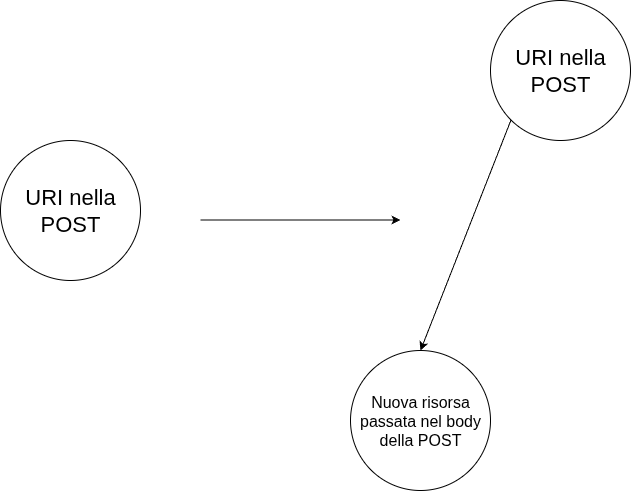
\includegraphics[scale=0.275]{img/metodoPOST.png}
    \end{figure}
    Sarà quindi responsabilità del server trovare un nuovo URI per la nuova risorsa.
    \newpage
    \item \textbf{PUT/DELETE}: Permette di inserire (PUT) o cancellare (DELETE) una risorsa all'URI passato al metodo.
    \begin{enumerate}
        \item \textbf{Sintassi}: $\boxed{\text{PUT/DELETE} \:\: [RISORSA]}$
    \end{enumerate}
    In questo caso invece il client dovrà conoscere a priori l'URI della nuova risorsa che sta inserendo.
\end{enumerate}

\paragraph{Metodi Safe ed Idempotenti} Definiamo queste due proprietà e listiamo i metodi che le rispettano:

\begin{enumerate}
    \item \textbf{Metodi Safe}: Non hanno effetti collaterali, dunque non modificano la risorsa, quindi i metodi: GET, HEAD, OPTION e TRACE.
    \item \textbf{Metodi Idempotenti}: Hanno lo stesso effetto se eseguiti una o $n$ volte sulla stessa risorsa, quindi i metodi: GET, HEAD, PUT, DELETE, OPTION, TRACE. 
\end{enumerate}

\subsubsection{Web Caching}

Immaginando di avere una rete locale, assumendo di avere \{$host_1, ... , host_k$\} nella rete, cosa succede se $host_1$ richiede una risorsa
su un host remoto $host_x$ e lo stesso viene fatto da $host_2$ subito dopo? Questo procedimento attualmente non viene per nulla ottimizzato, di conseguenza
sono state formulate politiche di caching che permettono, tramite l'utilizzo di host intermedi, di mantenere le informazioni riguardanti le richieste per non ripeterle.

\begin{enumerate}
    \item \textbf{Server Proxy}: Un approccio di \textbf{Web Caching} infatti è quello del \textbf{Server Proxy}, che si pone tra gli host della rete locale ipotizzata ed il server remoto. Se il server proxy cachasse infatti le richieste
    allora il secondo host potrebbe acquisire quelle infomazioni senza effettuare richieste al server remoto ma solo richiedendole al server proxy stesso.
    \item \textbf{User Agent Cache}: Un metodo alternativo è quello che si basa sul mantenimento in locale da parte del browser delle risorse visitate da un utente.
\end{enumerate}

\subsubsection{Cookies}

Il protocollo HTTP è per definizione stateless, di conseguenza risulta necessario un meccanismo che permetta di
mantenere uno stato utente riguardante la sua navigazione su una applicazione web. Vengono quindi utilizzati per autenticazione, ricordare il profilo utente e creare sessioni su un protocollo stateless.

\vspace*{10px}

Si vuole quindi avere la possibilità di numerare e far riconoscere gli utenti sul sito presentando ogni volta un cookie.
Il meccanismo nello specifico si basa su questi passaggi:

\begin{enumerate}
    \item \textbf{Riga di intestazione} nel \textbf{messaggio di risposta} HTTP.
    \item \textbf{Riga di intestazione} nel \textbf{messaggio di richiesta} HTTP.
    \item \textbf{Cookie file} mantenuto dal \textbf{browser} dell'user.
    \item \textbf{Database} di gestione \textbf{cookie} del \textbf{server web}.
\end{enumerate}

\newpage

\paragraph{Cookie First/Third Party} Esistono due tipologie diverse di cookie:

\begin{enumerate}
    \item \textbf{First Party Cookie}: Creati direttamente dal sito web che l'utente sta visitando per mantenere informazioni riguardanti lo stato.
    \item \textbf{Third Party Cookie}: Memorizzano informazioni sensibili riguardanti gli utenti, sono creati e memorizzati da un dominio diverso rispetto a quello del sito web visitato.
\end{enumerate}

\subsection{Protocollo Telnet}

Protocollo di terminale il cui scopo è quello di permettere l'uso interattivo di macchine remote.
Chiaramente i due calcolatori devono poter comunicare a prescindere dai sistemi operativi che utilizzano, di conseguenza si utilizza un \textbf{interfaccia minima} a \textbf{caratteri}.

\paragraph{Protocollo TELNET [RFC 854]} Questo modello standardizzato si basa su un programma client ed uno server, nello specifico si seguono questi passi:

\begin{enumerate}
    \item Il client stabilisce una \textbf{connessione TCP} con il server.
    \item Il \textbf{client} acquisisce l'\textbf{input dei tasti} e lo invia al server, successivamente \textbf{accetta i caratteri} che il \textbf{server manda indietro} e li visualizza sul terminale utente.
    \item Il server accetta la connessione TCP e trasmette i dati al sistema operativo locale.
\end{enumerate}

Il client si connette alla porta $23$ del server e la connessione TCP persiste per la durata della sessione di login.

\paragraph{NVT - Network Virtual Terminal} L'obiettivo di TELNET è quello di poter operare con quanti più calcolatori diversi e di conseguenza sistemi operativi eterogenei. Di conseguenza si definisce un
\textbf{terminale virtuale} che permette la conversione dei comandi dei vari terminali locali e viceversa, creando una vera e propria interfaccia comune di riferimento. Si definiscono quindi dei set di caratteri universali per trasformare quelli delle macchine locali in comunicazione tra loro.

\paragraph{SSH - Secure Shell} Lo standard attuale per comunicazioni tra macchine remote via terminale è SSH, ossia un architettura di protocolli nata per sostituire TELNET ed i suoi problemi di sicurezza. Uno dei servizi principali di SSH è quello di tunneling, infatti grazie al port forwarding
possiamo mettere in comunicazione due processi su due macchine diverse mappando le loro porte a quella di SSH, lasciando quindi viaggiare la comunicazione tra i due processi tramite il tunnel SSH.

\newpage

\subsection{Protocollo SMTP - Simple Mail Transport Protocol}

Uno dei protocolli applicativi più antichi, si basa su due "protagonisti":

\begin{enumerate}
    \item \textbf{User Agent}: Client dell'user che permette l'editing e l'invio di messaggi di posta.
    \item \textbf{Mail Server}: Server dei provider che devono archiviare i messaggi ricevuti, dato che il tipo di comunicazione tra i vari User Agent è asincrona, di conseguenza dovranno immagazzinare in una coda i messaggi in uscita.
\end{enumerate}

\paragraph{Indirizzo Mail - Sintassi} Solitamente un indirizzo è indicato con:

\[ \boxed{\text{local-part} \: @ \: \text{domain-name}} \]

\vspace*{5px}

dove con \textit{local-part} si indica la specifica "cassetta" dell'user nel mail server, mentre
\textit{domain-name} indica l'effettivo mail server.

\paragraph{Spooling dei Mail Server} I Mail Server seguono una tecnica di spooling, ossia tentano di inviare i messaggi di posta settando una connessione TCP con la macchina destinazione. Se la connessione viene aperta e il trasferimento va a buon fine allora
il Mail Server cancella la copia della mail in locale. Altrimenti, se qualcosa dovesse andare storto ritenterebbe la connessione TCP in maniera periodica fino ad un certo intervallo di tempo, se viene superato allora si scarta il messaggio, notificando il mittente della condizione.

\paragraph{Gestione Alias dei Mail Server} Gestione a puntatori di indirizzi di casella postale, ne esistono di due tipi:

\begin{enumerate}
    \item \textbf{Uno a Molti}: Un singolo indirizzo alias riferisce a più indirizzi mail reali.
    \item \textbf{Molti a Uno}: Un singolo indirizzo mail reale ha molti indirizzi alias che lo riferiscono.
\end{enumerate}

\paragraph{Protocollo SMTP [RFC5321]} Si stabilisce una connessione TCP sulla porta $25$, si segue una politica PUSH da parte di ogni client fino a quello precedente al destinatario. Quindi
dal primo user fino all'ultimo Mail Server tutti agiranno da client nei confronti del server destinatario successivo. Tre fasi:

\begin{enumerate}
    \item Handshaking a livello applicativo.
    \item Trasferimento messaggi in coda.
    \item Chiusura.
\end{enumerate}

\vspace*{-10px}

\subparagraph{Comandi SMTP} Questo standard definisce specifici comandi:

\begin{enumerate}
    \item $\text{HELO} \: < \text{client identifier} > $
    \item $\text{MAIL FROM:} \: < \text{reverse-path} > \: < \text{CRLF} > $
    \item $\text{RCPT TO:} \: < \text{forward-path} > \: < \text{CRLF} > $
    \item $\text{DATA}$
    \item $\text{QUIT}$
\end{enumerate}

\newpage

\paragraph{Formato Messaggi SMTP}

I comandi sono formato ASCII, mentre le risposte sono ASCII a 7 bit. Nello specifico, il messaggio è così composto:

\begin{enumerate}
    \item \textbf{Header}: Contiene le linee d'intestazione, come ad esempio \textit{To}, \textit{From}, \textit{Subject}, che \textbf{non} corrispondono ai parametri passati ai comandi SMTP citati prima. 
    \item \textbf{Body}: Contiene il messaggio effettivo, composto da caratteri ASCII a 7 bit.
\end{enumerate}

\paragraph{MIME - Multipurpose Internet Mail Extension} Fino ad ora i body erano composti solo da caratteri ASCII a 7 bit. Si definisce quindi una codifica per trasferimento media e testo non-ASCII.
Si aggiungono quindi dei parametri nelle intestazioni per dichiarare l'utilizzo del MIME nel body.

\subsection{Protocolli POP3/IMAP}

Fino ad ora abbiamo descritto il protocollo SMTP che pusha l'informazione fino all'ultimo mail server. Essendo però un tipo di comunicazione asincrona, sarà il client del destinatario a pullare il messaggio. Si definiscono quindi i protocolli
POP e IMAP.

\begin{enumerate}
    \item \textbf{POP3}: Il client apre una connessione TCP sulla porta 110, si autentica con utente e password e richiede l'elenco dei messaggi e li preleva uno alla volta.
    \item \textbf{IMAP}: Più feature di POP3, permette la gestione logica in folder dei messaggi memorizzati sul server e permette di estrarre solo alcuni componenti dei messaggi.
    \item \textbf{HTTP}: In alternativa, anche HTTP può effettuare richieste ai Mail Server tramite browser.
\end{enumerate}

\subsection{DNS - Domain Name System}

Vogliamo avere la possibilità di dereferenziare nomi e non indirizzi numerici, dato che questi ultimi risultano essere più difficili da ricordare. La domanda quindi è come \textbf{associare indirizzi IP a nomi}.
Inizialmente la gestione di queste associazioni era statica, ma attualmente risulta impossibile utilizzare questa politica, date le dimensioni di Internet.

\paragraph{Architettura Centralizzata vs Distribuita} Potremmo immaginare un unico server con relativo unico database a cui riferirsi per risolvere queste associazioni. Questo però ci vincolerebbe ad una \textbf{pesante dipendenza} da quest'ultimo. Questo dovrebbe gestire miliardi di query al giorno, ed in caso di fallimento del server si bloccherebbe tutto Internet. Si preferisce quindi un architettura distribuita.

\paragraph{Composizione Essenziale del DNS} Si compone di tre elementi fondamentali:

\begin{enumerate}
    \item Uno \textbf{schema di assegnazione} dei \textbf{nomi} gerarchico basato sui domini.
    \item Un \textbf{database distribuito} contenente nomi e corrispondenti IP.
    \item Un \textbf{protocollo} per la \textbf{distribuzione delle informazioni} tra \textbf{name servers}:
    \begin{enumerate}
        \item \textbf{Name Servers}: Comunicano per risolvere nomi.
        \item \textbf{Porta}: Utilizzano porta 53 in UDP (sono a volte TCP).
    \end{enumerate}
\end{enumerate}

\newpage

\paragraph{Servizi Offerti dal DNS} Elenchiamo i servizi offerti dal DNS:

\begin{enumerate}
    \item Risoluzione nomi (hostnames) in indirizzi IP.
    \item \textbf{Host Aliasing}: Più alias possono dereferenziare lo stesso hostname, e di conseguenza, lo stesso indirizzo IP.
    \item \textbf{Distribuzione Carico}: In caso di potenziale carico elevato assegnato ad un server, si fa corrispondere un singolo hostname a più IP per evitare problemi di sovraccarico su una macchina specifica.
    
\end{enumerate}

\paragraph{Struttura Gerarchica di Gestione Domini} Lo spazio dei nomi è definito da una \textbf{struttura gerarchica ad albero} dove ogni nodo è identificato da un \textbf{etichetta}, ossia un \textbf{nome di dominio}.

\begin{figure}[htbp]
    \center
    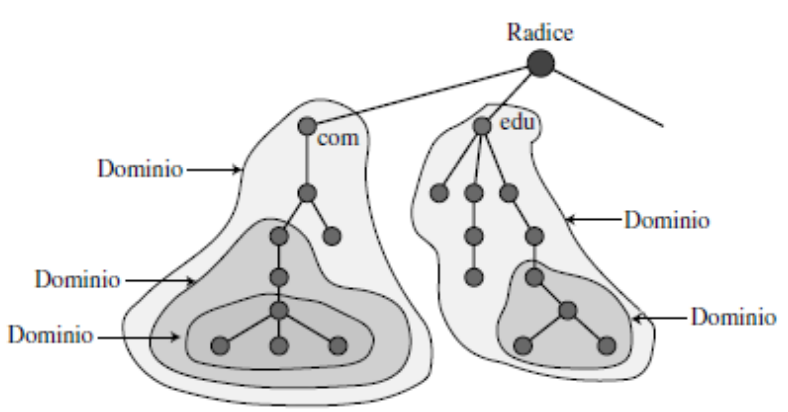
\includegraphics[scale=0.5]{img/DNS1.png}
\end{figure}

I domini top-level (.com, .edu, .gov, .net, .org) vengono gestiti dallo IANA.

\subsubsection{Gerarchia dei Name Servers}

Avendo definito il \textbf{DNS} come un \textbf{database distribuito} in una \textbf{gerarchia} di più \textbf{name servers}, allora bisogna definire cosa sia un \textbf{name server}, ossia un 
programma che gestisce la conversione da nome di dominio ad indirizzo IP.

\paragraph{Zone e Domini di Name Servers} Tutte le informazioni per le risoluzioni di nomi sono ripartite su più name server, dunque ciascuno di essi immagazzina le info relative alla propria \textbf{zona} ed i riferimenti ai \textbf{name servers} dei \textbf{domini} di \textbf{livello inferiore}.

\vspace*{10px}

\begin{figure}[htbp]
    \center
    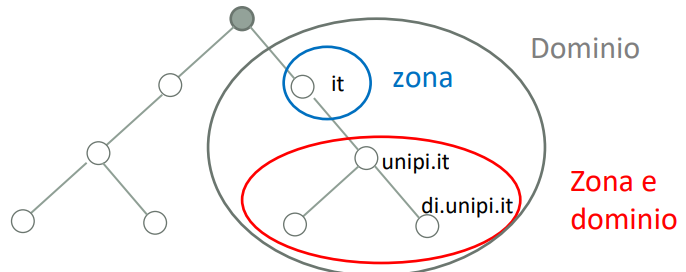
\includegraphics[scale=0.5]{img/DNS2.png}
\end{figure}

\newpage

\paragraph{Ruoli dei Server nella Gerarchia} Elenchiamo tutti i ruoli e le loro responsabilità:

\begin{enumerate}
    \item \textbf{Root Name Server}: Responsabile dei record della zona radice, riconosce tutti i domini TLD (Top Level Domain) e conosce il server TLD che li risolve, quindi restituisce le info sui name server TLD. A questo ruolo corrispondono circa 13 indirizzi IP.
    \item \textbf{Top Level Domain Server}: Mantiene le info dei nomi di dominio che appartengono ad un certo TLD, e restituisce informazioni sui name server di competenza dei sottodomini.
    \item \textbf{Authoritative Name Server}: Responsabile di una certa \textbf{zona}, memorizza nome ed indirizzo IP di un insieme di host di cui può effettuare la traduzione. Questo ruolo può essere suddiviso in altri due sottoruoli:
    \begin{enumerate}
        \item \textbf{Primary Authoritative Name Server}: Mantengono il file di zona.
        \item \textbf{Secondary Authoritative Name Server}: Ricevono il file di zona e offrono il servizio di risoluzione.
    \end{enumerate}
\end{enumerate}

A questa gerarchia si \textbf{aggiunge} un \textbf{ulteriore ruolo}, che \textbf{non appartiene} propriamente alla \textbf{gerarchia}, ma che si occupa da prima interfaccia nel caso in cui un client (es. Browser) tenti di riferire ad un nome:

\begin{enumerate}
    \item \textbf{Local Name Server}: Un server appartenente ad un ISP (Internet Service Provider) che assume il ruolo di proxy, per fare prima un controllo nelle tabelle locali per cercare la risoluzione del nome richiesto dal client, e solo successivamente, in caso di fault, richiede
    la query effettiva al DNS, nello specifico ad un Root Name Server.    
\end{enumerate}

\vspace*{-10px}

\paragraph{Query Ricorsiva/Iterativa} Esistono due tipi diversi di risoluzione dei nomi:

\begin{enumerate}
    \item \textbf{Query Ricorsiva}: Il Local Name Server richiede una conversione completa di nome.
    \item \textbf{Query Iterativa}: Viene restituito al client o al Local Name Server il riferimento al server successivo da contattare per completare la risoluzione di nome.
\end{enumerate}

\vspace*{-20px}

\begin{figure}[htbp]
    \centering
    \begin{minipage}{0.35\textwidth}
        \centering
        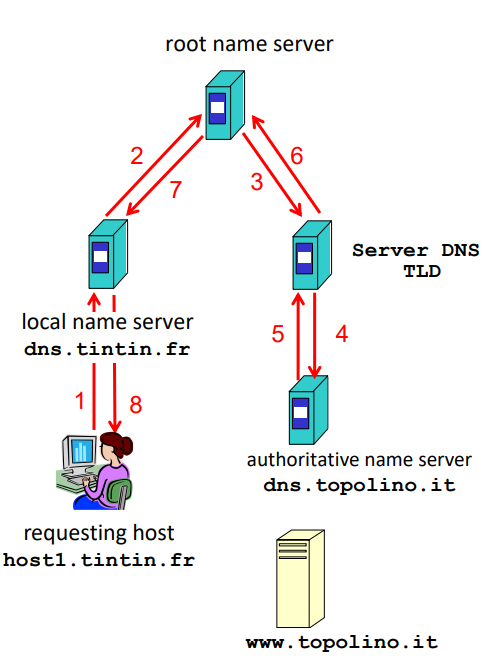
\includegraphics[width=\linewidth]{img/queryRicorsiva.png}
        \caption{Query Ricorsiva}
    \end{minipage}
    \hspace{0.8cm}  
    \begin{minipage}{0.37\textwidth}
        \centering
        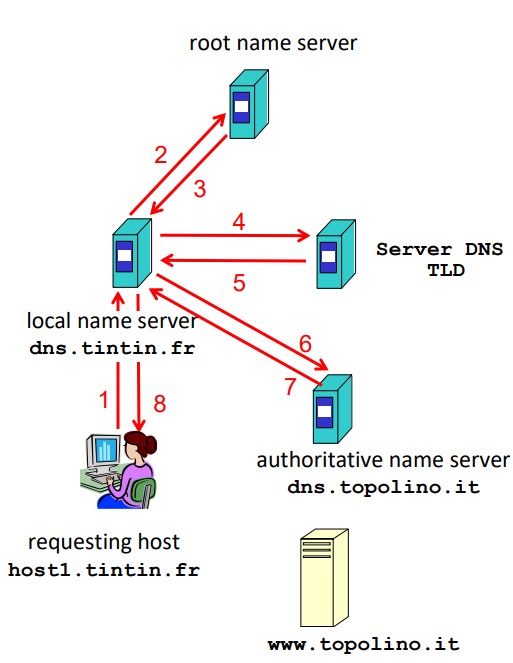
\includegraphics[width=\linewidth]{img/queryIterativa.png}
        \caption{Query Iterativa}
    \end{minipage}
\end{figure}

\newpage

\paragraph{Caching DNS} Nel DNS si utilizza molto il caching per ridurre richieste che rimbalzano continuamente tra server. Solitamente quindi si mantiene in cache di server DNS il dato in cache in modo non autorevole, e i server invalideranno queste informazioni dopo un periodo fissato. Un altro approccio potrebbe essere quello di mantenere in cache direttamente degli indirizzi 
IP di server DNS TLD (Top Level Domain), evitando di riferirsi più volte ai server radice.

\paragraph{Record DNS} Un DNS è un database distribuito di \textit{resource records} (RR) che seguono la seguente sintassi:

\[ \boxed{\text{RR format}: \:\: ( \text{name, value, type, ttl})} \]

\vspace*{10px}

dove gli elementi vengono così interpretati:

\begin{enumerate}
    \item \textbf{TTL}: Tempo residuo del record in cache.
    \item \textbf{Name} e \textbf{Value}: Dipendono da type.
    \item \textbf{Type}: Esistono vari tipi:
    \vspace*{5px}
    \begin{center}
        \begin{tabular}{|l|l|p{0.45\textwidth}|}
        \hline
        \textbf{Type} & \textbf{Name} & \textbf{Value} \\
        \hline
        A & hostname & indirizzo IP \\
        \hline
        CNAME & hostname (sinonimo) & nome canonico dell'host \\
        \hline
        NS & nome di dominio & hostname dell'Authoritative Name Server per quel dominio \\
        \hline
        MX & nome di dominio & nome canonico del server di posta associato a name \\
        \hline
        \end{tabular}
    \end{center}
\end{enumerate}

\vspace*{15px}

\subsubsection{Protocollo DNS}

L'effettivo protocollo del livello applicazione che si occupa di questa risoluzione di nomi utilizza prevalentemente \textbf{UDP} sulla \textbf{porta 53}.
L'applicazione è detta \textbf{resolver}, effettua polling al server DNS e dopo $n$ richieste o richiede ad un altro server oppure informa l'applicazione con il fallimento.

\vspace*{10px}

\paragraph{Perchè UDP e Quando TCP} Viene utilizzato il protocollo TCP per una questione di riduzione di ritardi, riduzione di overhead causato dal setup di TCP e perchè solitamente le query DNS richiedono pochi dati, quindi rispettano le dimensioni di un pacchetto UDP. A volte viene utilizzato il protocollo TCP, ma questo
accade solo se è necessaria l'affidabilità del trasferimento oppure se si sforano i $512$ byte dei pacchetti UDP.

\newpage

\paragraph{Messaggi del Protocollo DNS} I messaggi di query e reply seguono lo stesso formato:

\begin{figure}[htbp]
    \center
    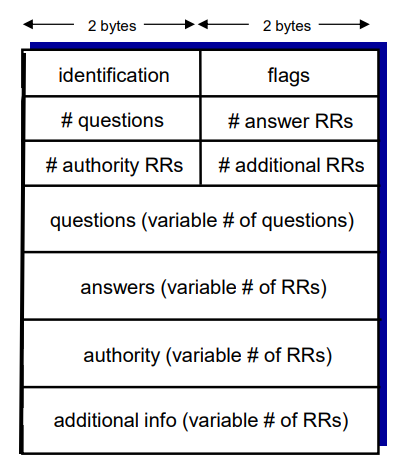
\includegraphics[scale=0.65]{img/messaggioDNS.png}
\end{figure}

Dove ogni campo indica

\begin{enumerate}
    \item \textbf{Identification}: Campo di $16$ bit per l'identificazione di una query, la risposta ad una query usa lo stesso identification id.
    \item \textbf{Flags}: Indicano se query o reply, se desiderata o disponibile la ricorsione e se la risposta è autorevole.
    \item \textbf{Questions}: Nome richiesto e tipo di query.
    \item \textbf{Answers}: RR (\textit{resource records}) in risposta alla query.
    \item \textbf{Authority}: Record per i server di competenza.
    \item \textbf{Additional Info}: Informazioni utili aggiuntive.
\end{enumerate}

\paragraph{DNS e Sicurezza} Dato il funzionamento molto decentralizzato del DNS, esistono vari attacchi che sfruttano questa sua caratteristica:

\begin{enumerate}
    \item \textbf{DNS Cache Poisoning}: Un attaccante invia risposte DNS falsificate ad un DNS Server o ad un client, avvelenandone la cache.
    \item \textbf{Man-in-the-Middle Attack}: Vengono intercettate le comunicazioni tra un client ed un server DNS, ed in questo modo viene indirizzato un obiettivo verso host malevoli.
    \item \textbf{DNS Hijacking}: Si restituiscono risposte non corrette alle query DNS, reindirizzando il client verso siti malevoli alterando le impostazioni DNS. Questo può essere fatto
    a diversi livelli, infatti può essere un Local, Router oppure Rogue Hijacking.
\end{enumerate}

\newpage

\section{Livello Trasporto}

L'obiettivo di questo livello è quello di creare una connessione logica tra processi applicativi su host diversi, assumono quindi di essere collegati a livello fisico, astraendo dalla reale connessione fisica di cui si occuperanno i livelli sottostanti. I protocolli di trasporto vengono
eseguiti nei sistemi terminali, mantenendo la politica per cui si mantengono dumb i dispositivi intermedi e smart quelli terminali.

\subsection{Introduzione al Livello Trasporto}

In questo sottocapitolo definiamo concetti base del livello trasporto.

\paragraph{Servizi del Livello Trasporto} Elenchiamo i servizi offerti da questo livello:

\begin{enumerate}
    \item Offre servizi al livello applicazione, permettendo alle applicazioni di scegliere il modo in cui inviare/ricevere dati secondo uno \textbf{stile} a \textbf{messaggi} oppure a \textbf{stream}.
    \item Comunica con il livello Rete sottostante, che si occupa a sua volta della consegna del datagramma all'host destinatario. 
\end{enumerate}

\paragraph{Servizio Connection/Non Connection Based} Seguendo gli stili definiti sopra possiamo definire anche servizi orientati o meno alla connessione. Nello stile orientato alla connessione
si instaura una logica di server/client dopo una fase di setup, mentre in uno stile non orientato alla connessione i dati vengono visti come messaggi indipendenti.

\paragraph{Azioni del Livello Trasporto} Elenchiamo le azioni di questo livello in base a chi le esegue:

\begin{enumerate}
    \item \textbf{Azioni Mittente}:
    \begin{enumerate}
        \item Riceve un messaggio dal livello applicazione.
        \item Determina i valori dell'header del segmento.
        \item Crea il segmento.
        \item Passa il segmento al livello Rete.
    \end{enumerate}
    \item \textbf{Azioni Destinatario}:
    \begin{enumerate}
        \item Riceve il segmento dal livello Rete.
        \item Controlla i valori dell'header.
        \item Estrae il messaggio del livello applicazione.
        \item Smista il messaggio all'applicazione attraverso la socket.
    \end{enumerate}
\end{enumerate}

\newpage

\subsection{TCP vs UDP e Multiplexing/Demultiplexing}

I due protocolli di trasporto principali hanno caratteristiche differenti:

\begin{enumerate}
    \item \textbf{Protocollo TCP}:
    \begin{enumerate}
        \item Orientato alla Connessione.
        \item Orientato allo Stream.
        \item Gestione della connessione.
        \item Consegna affidabile dei dati.
        \item Controlli di congestione e flow.
    \end{enumerate}
    \item \textbf{Protocollo UDP}:
    \begin{enumerate}
        \item Senza connessione, non affidabile.
        \item Orientato al messaggio.
        \item Estensione del servizio \textit{host to host} del livello rete.
    \end{enumerate}
\end{enumerate}

Entrambi i protocolli però offrono controlli sugli errori e servizi di multiplexing e demultiplexing.

\paragraph{Multi/Demultiplexing} Il livello di trasporto ha la responsabilità di smistare i messaggi ottenuti dal livello di rete tra i vari processi tramite la risoluzione di socket address.
Questo risulta necessario se più processi utilizzano lo stesso protocollo di trasporto per la comunicazione su rete, cosa che accade molto spesso. Quindi abbiamo due attori duali:

\begin{enumerate}
    \item \textbf{Mittente in Multiplexing}: Gestisce i dati da più socket e si occupa dell'aggiunta del header di trasporto.
    \item \textbf{Destinatario in Demultiplexing}: Usa le informazioni nell'header per recapitare i segmenti alla corretta socket.
\end{enumerate}

Nello specifico, nel demultiplexing vengono utilizzati dall'host indirizzi IP e numeri di porta per smistare il segmento verso la corretta socket dato che ogni datagramma si porta dietro un segmento del
livello trasporto ed ogni segmento nell'header mantiene un numero di porta sorgente ed uno di destinazione.

\paragraph{Definizione di Porta} Ogni comunicazione a livello trasporto è univocamente identificata tramite la combinazione $IP/porta$, una \textbf{porta} è quindi definita come un intero a $16$ bit che viene assegnato
ad un processo, più nello specifico è un \textbf{punto di demultiplexing} dei protocolli TCP o UDP. Esistono dei range di porte predefinite, come le \textit{System Ports}, \textit{User Ports} o \textit{Dynamic Ports}. In generale è il
sistema operativo ad occuparsi dell'assegnamento di porte.

\paragraph{Multiplexing TCP/UDP} Esistono differenze tra i tipi di multiplexing dei due protocolli, infatti il protocollo TCP esegue il multiplexing basandosi su una quadrupla con tutte le informazioni su sorgente e destinatario
ossia $(IP_{sorg}, porta_{sorg}, IP_{dest}, porta_{dest})$, mentre il protocollo UDP utilizza la coppia $(IP_{dest}, porta_{dest})$.

\newpage

\subsection{Trasporto UDP}

Servizio di trasporto best effort, i datagrammi UDP possono essere persi o consegnati fuori sequenza. Questo protocollo è orientato al messaggio, quindi ogni datagramma è indipendente e di dimensioni limitate.
Questo garantisce però una semplicità non indifferente, risultando vantaggioso in contesti di applicazioni time-sensitive.

\paragraph{Impieghi e Caratteristiche del Trasporto UDP} E' facile e leggero da gestire, non esiste alcun controllo sulla congestione e le intestazioni non superano gli $8$ byte. Viene impiegato in contesti di applicazioni multimediali, dove sono tollerate le piccole perdite, oppure in altre applicazioni come il DNS, HTTP/3 o SNMP (Simple Network Management Protocol).

\paragraph{Azioni Mittente/Destinatario} Elenchiamo le azioni effettuate in base al tipo di attore:

\begin{enumerate}
    \item \textbf{Azioni Mittente}:
    \begin{enumerate}
        \item Riceve un messaggio del livello Applicazione.
        \item Determina i valori dei campi dell'header UDP.
        \item Crea lo user datagram.
        \item Passa lo user datagram al livello Rete.
    \end{enumerate}
    \item \textbf{Azioni Destinatario}:
    \begin{enumerate}
        \item Riceve lo user datagram dal livello Rete.
        \item Controlla la checksum
        \item Estrae il messaggio di livello Applicazione.
        \item Smista il messaggio attraverso la socket.
    \end{enumerate}
\end{enumerate}

\paragraph{Composizione di un Datagramma UDP} Descriviamo l'entità base del protocollo UDP:

\vspace*{10px}

\begin{center}
    \begin{tabular}{|l|l|}
    \hline
    numero porta sorgente & numero porta destinazione \\
    \hline
    lunghezza & checksum \\
    \hline
    \multicolumn{2}{|c|}{\rule{0pt}{3em}payload\rule{0pt}{3em}} \\
    \hline
    \end{tabular}
\end{center}

\vspace*{10px}

Il messaggio si compone di $8$ byte di intestazione, i numeri di porta per la fase di demultiplexing e la lunghezza del messaggio massima del datagramma UDP è di $65535$ byte.

\newpage

%\begin{figure}[htbp]
    %\center
    %\includegraphics[scale=0.4]{img/classiComplessita2.png}
%\end{figure}


\end{document}